\chapter{User Manual}
\label{ch:manual}
This chapter will have the user manual.
\section{UI/UX}
These UI/UX elements are crafted to be responsive and visually appealing, ensuring a seamless and enjoyable experience for users as they practice medical procedures and scenarios.
\section{Choose Scenario}
The user interface (UI) enhances the user experience (UX) with intuitive design elements. Users start by selecting a scenario corresponding to a patient's medical issue from a menu of various conditions or scenarios.
\begin{figure}[h]
    \centering
    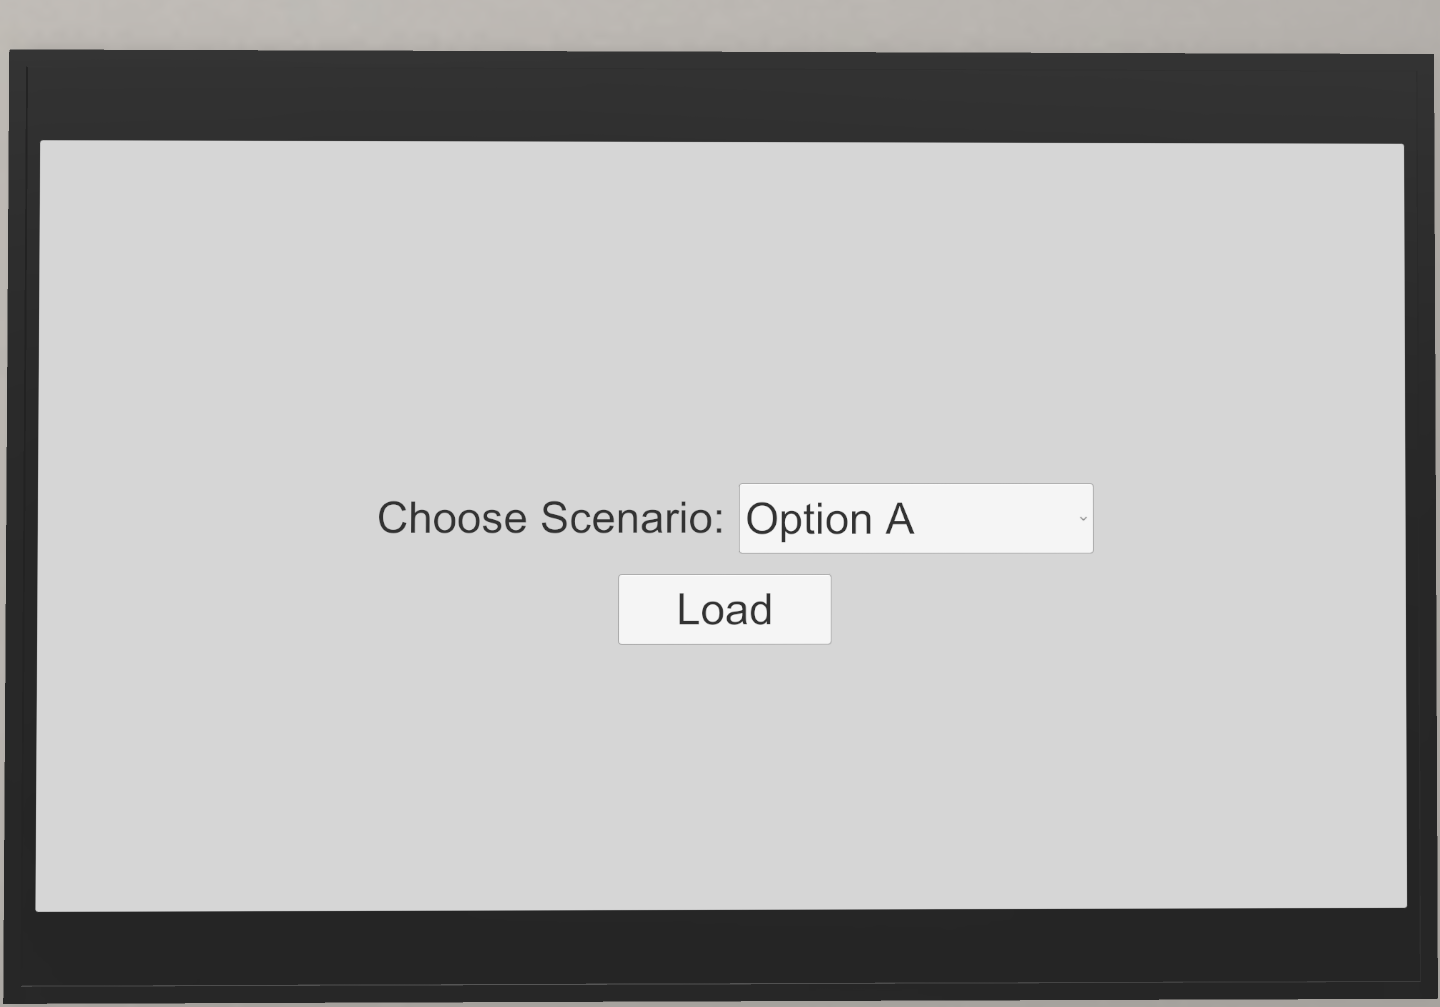
\includegraphics[width=0.5\linewidth]{Images/screen.png}
    \caption{Choose Scenario}
    \label{fig:ChooseScenario}
\end{figure}
\section{1.1 Toggle Menu}
Once a scenario is chosen, the UI features a 1.1 toggle menu for keyboard interaction, enhancing user engagement.
\begin{center}
    {Toggle Control Hints:} \textbf{F1} \\ 
    {Move Player/Playspace:} \textbf{WASD} \\
    {Sprint Modifier:} \textbf{(LeftShift)} \\
    {Mouse:} HMD Rotation \\
    {Modes:} Controller \textbf{(LeftAlt)} \\
    {Distance Pickup Modifier:} \textbf{(LeftControl)} \\
    {Distance Pickup Left Hand:} \textbf{(Mouse0)} \\
    {Distance Pickup Right Hand:} (\textbf{(Mouse1)}
\end{center}
\section{1.2 Toggle Menu}
Additionally, the project features a more options toggle menu that offers expanded functionalities and settings. This collapsible menu shows keyboard interactions in more detail.
\begin{center}
        {Toggle Control Hints:} \textbf{F1} \\
        {Move Player/Playspace:} \textbf{WASD} \\
        {Sprint Modifier:} \textbf{(LeftShift)} \\
        {Mouse:}\textbf{ Controller Position} \\
        {Modes:} HMD \textbf{(LeftAlt)}, Rotation \textbf{(LeftShift)} \\
        {Controller Hand:} Right \textbf{(Tab)} \\
        {Axis:} X/Z \textbf{(LeftControl)} \\
        {Button Press Mode Modifiers:} Touch \textbf{(T)}, Hair Touch \textbf{(H)} \\
        {Trigger Press:} \textbf{Mouse1} \\
        {Grip Press:} \textbf{Mouse0} \\
        {Touchpad Press:} \textbf{Q} \\
        {Button One Press:} \textbf{E} \\
        {Button Two Press:} \textbf{R} \\
        {Start Menu Press:} \textbf{F}
\end{center}